\documentclass[11pt]{article}
\usepackage[utf8]{inputenc}

\usepackage[left=2.5cm,top=2.5cm,right=2.5cm,bottom=2.5cm]{geometry}
\usepackage{times} % font type
\usepackage{url} % for clickable web addresses in PDF document
\usepackage{graphicx} % for figures
\usepackage{float} % to force figure or table here [H]
\usepackage{multirow} % For tables with different rows and columns

\title{Precision medicine and quantitative imaging in prostate cancer \\ - a multiscale approach}
\author{OERCompBiomed Summer School, Seili, 11-16 August 2019}
\date{GROUP \#x  - yy August 2019}

\begin{document}

\maketitle

\begin{scriptsize}
\noindent \underline{DESCRIPTION OF THE ASSIGNMENT}: \, {\it Imagine that you are a group of established successful scientists that will team up to tackle an important biomedical and medical challenge. There is an open call for research proposals under a new umbrella program entitled “Artificial intelligence and computational (bio)medicine”, where your multidisciplinary group are aiming for a project on “Precision medicine and quantitative imaging in prostate cancer - a multiscale approach”.  
We assume you obtain (or already have) some knowledge about prostate cancer (PCa), e.g.}

\begin{center}
\begin{itemize}
    \item \url{https://en.wikipedia.org/wiki/Prostate_cancer}
    \item \url{https://www.cancer.org/cancer/prostate-cancer}
    \item \url{https://prostatecancerfree.org/prostate-cancer-videos}
    \item \url{http://pathology.jhu.edu/ProstateCancer}
    \item \url{https://www.science.gov/topicpages/c/cancer+gleason+score}
\end{itemize}
\end{center}


{\it Regarding imaging, there are a lot of available {\bf data in repositories} e.g.}


\begin{center}
\begin{itemize}
    \item \url{https://prostatex.grand-challenge.org}
    \item \url{https://wiki.cancerimagingarchive.net/display/Public/SPIE-AAPM-NCI+PROSTATEx+Challenges}
    \item \url{https://promise12.grand-challenge.org}
    \item \url{https://www.aapm.org/GrandChallenge/PROSTATEx-2}
    \item \url{https://wiki.cancerimagingarchive.net/display/Public/Prostate+Fused-MRI-Pathology}
\end{itemize}
\end{center}


{\it and  computational methods and {\bf software code} from the field of machine learning (incl radiomics, deep learning), e.g.}

\begin{center}
\begin{itemize}
    \item \url{https://github.com/oercompbiomed/CBM101}
    \item \url{https://github.com/eiriniar/gleason_CNN}
    \item \url{https://github.com/mirzaevinom/prostate_segmentation}
    \item \url{https://ai.googleblog.com/2018/11/improved-grading-of-prostate-cancer.html}
    \item \url{https://github.com/SlicerProstate/SliceTracker}
    \item \url{https://www.ncbi.nlm.nih.gov/pmc/articles/PMC5703221}
    \item \url{https://github.com/SlicerProstate/SliceTracker}
    \item \url{https://github.com/anirudhtomer/prias}
    \item \url{https://github.com/Wenyuan-Vincent-Li/Path_R_CNN}
    \item \url{https://github.com/Radiomics/pyradiomics}
\end{itemize}
\end{center}


 {\it and you are encouraged to use or refer to these in your project.}\\
 
 \noindent {\it The focus of the assignment is (i) description of relevant imaging technologies and modalities - at different scales, (ii) proposal of imaging-derived biomarkers for PCa, (iii) machine learning techniques for classification, treatment stratification and prediction, (iv) the novelty and impact of your approach, and (v) the evaluation of the ethics of your project - and not so much the scientific background of prostate cancer per se.}

\end{scriptsize}


\section{Research plan} % 3-5 pages incl. figures and bibliography

\vspace{3mm}

\subsection{A brief background to the field}

\vspace{5mm}

\begin{quote} 
{\scriptsize \it  Example of describing a bibliographic reference and including a figure (check copyright status):}
\end{quote}

\noindent Recently, Chaddad et al. \cite{Chaddad2018} used quantitative imaging features derived from multiparametric MR image recordings and radiomic analysis in a machine learning framework to predict Gleason score in prostate cancer (cf. Fig.~\ref{fig:radiomic-model}).
 
\begin{figure}[H]
\centering
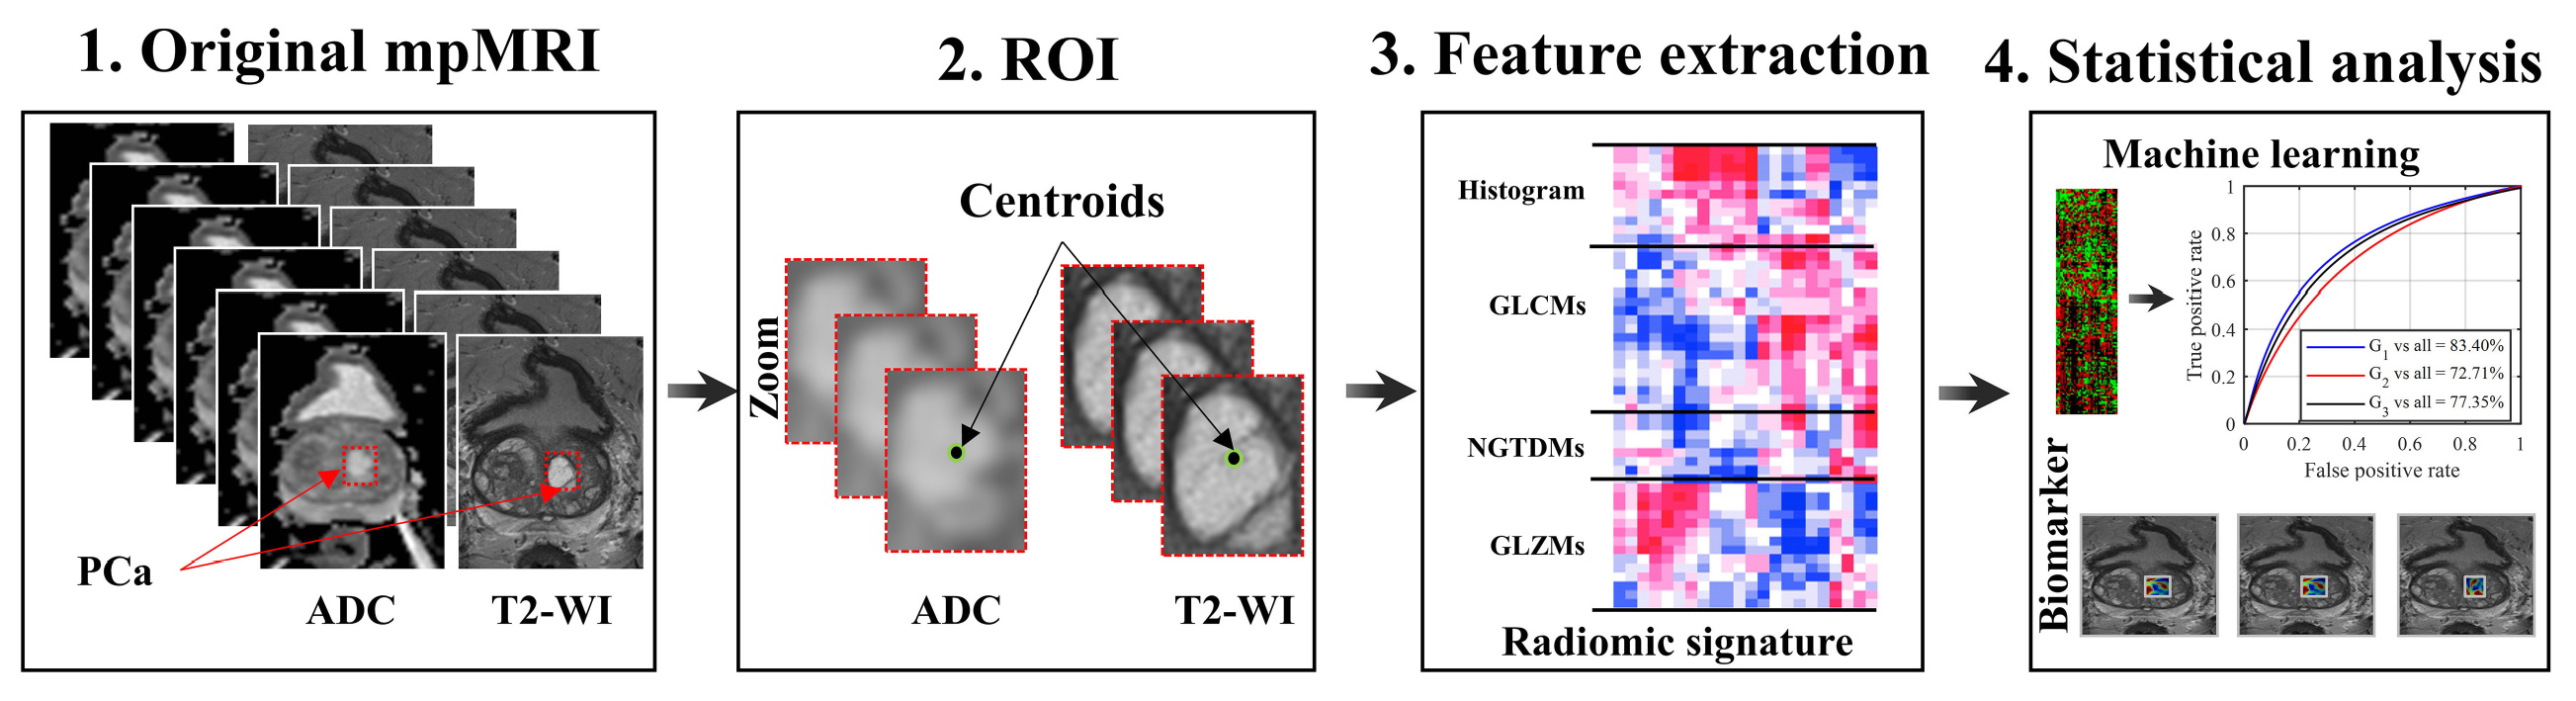
\includegraphics[width=0.98\linewidth]{chaddad_etal_2018_fig1.png} 
\vspace{-3mm}
\caption{\footnotesize Schema of a radiomic model for patients with PCa. Acquisition of pre-treatment PCa patient’s MR images; Regions of interest (i.e., subvolume $21 \times 21 \times 3$ voxels); Extraction of 41 radiomic features from ROIs; Feature significance analysis based on Spearman rank correlation and Kruskal-Wallis, and multivariate
prediction of Gleason score groups using the random forest model. {\scriptsize (Source: Chaddad A, Niazi T, Probst S, Bladou F, Anidjar M and Bahoric B (2018) Predicting Gleason Score of
Prostate Cancer Patients Using Radiomic Analysis.
Front. Oncol. 8:630. \protect\url{https://doi.org/10.3389/fonc.2018.00630} distributed under the terms of the Creative Commons Attribution License)}.}
\label{fig:radiomic-model}
\end{figure}

\vspace{5mm}

\begin{quote} 
{\scriptsize \it  Example of including a table:}
\end{quote}

For different imaging techniques, see Tab.~\ref{tab:imaging}.

% See https://www.overleaf.com/learn/latex/Tables
% here using multirow taking 3 parameters
% The first one is the number of rows to be combined, 3 in the example. 
% The second parameter is the width of the column, 4em in the example. 
% Finally, the third parameter is the content of the cell.
\begin{table}[H]
\begin{center}
\begin{tabular}{ |c|c|c|c| } 
\hline
{\bf Data acquisition} & {\bf Micro} & \multicolumn{2}{c|}{\bf Macro} \\
\hline
\multirow{3}{4em}{Imaging modalities} & {\it Optical} & {\it MRI}  & {\it PET} \\ 
& Opt-1 & MR-1  & PET-1\\ 
& Opt-2 & MR-2  & PET-2\\ 
\hline
\end{tabular}
\caption{Different imaging techniques for assessing PCa.}
\label{tab:imaging}
\end{center}
\end{table}


\subsection{Objectives and expected impact}

\vspace{3mm}

\subsection{Material and methods}

\begin{quote}
{\scriptsize \it A description of how you will use and integrate different imaging technologies and machine learning methodologies to improve diagnosis, treatment planning, follow-up and prognosis in PCa.}
\end{quote}

\vspace{3mm}

\subsection{Evaluation} 

\begin{quote}
{\scriptsize \it A description of the animal models / patient cohorts you will use to evaluate your methodological approach.}
\end{quote}

\vspace{3mm}

% See also: https://www.overleaf.com/learn/latex/Bibliography_management_in_LaTeX
% considering BibTeX / Jabref / Mendeley / Zotero / EndNote
% using BibTeX you can also edit the bib file directly via the files menu
\begin{thebibliography}{1} 
\bibitem{Chaddad2018}  Chaddad A, Niazi T, Probst S, Bladou F, Anidjar M and Bahoric B. Predicting Gleason Score of Prostate Cancer Patients Using Radiomic Analysis.
Front Oncol 2018;8:630. 
\end{thebibliography}

\newpage


\section{Data management plan and ethical considerations} % 1 1/2-2 1/2 pages incl. graphics / links

\begin{quote} 
{\scriptsize \it  The open science initiative encourages use of existing repositories and submitting new data and code being generated into repositories, to make study results widely available to the scientific community and improve reproducible research.
Write a separate data and code management plan that describes the data and code being used or generated in this study and how it is (or will be made) available. Include a separate section on ethical considerations (data collection and software development, restrictions on sharing of data and code, protection of privacy)}
\end{quote}

\vspace{3mm}

\subsection{Description of generated data and code}

\vspace{3mm}

\subsection{Sharing of data and code}

\vspace{3mm}

\subsection{Ethical considerations}

\end{document}
